\chapter{Arquitetura do \textit{middleware} de comunicação \label{chapter_middleware}}

Conforme mencionado no capítulo anterior, todo o desenvolvimento do \textit{framework} proposto neste trabalho se faz em cima de uma camada denominada \textit{middleware} de comunicação. Este capítulo descreve em detalhes a arquitetura do proposto \textit{middleware} de comunicação, tais como suas partes e suas principais funções: troca de mensagens e migração de processos lógicos. 

\section{Módulos do \textit{middleware}}

A arquitetura do \textit{middleware} é dividida em dois módulos principais: o ambiente (\textit{envinonment}) e o processo lógico (\textit{process}). Um ambiente representa um nó físico do sistema de simulação distribuída, ou seja, é a representação lógica de um computador no sistema distribuído. Em uma simulação distribuída, tipicamente, cada nó físico da rede deve conter um único \textit{environment}.

O segundo módulo da estrutura do \textit{middleware} é o processo lógico, que é a representação lógica de um processo no sistema de simulação distribuída. Na arquitetura aqui descrita, um processo lógico somente existe dentro de um \textit{environment}. Sendo assim, um \textit{environment} pode ser visto como um conjunto de processos lógicos. Por sua vez, um processo somente pode estar contido por um único \textit{environment} em um determinado momento.

Assim é definido:

Definição 1: Um \textit{environment} é um conjunto de processos.

Definição 2: Um processo só pode estar contido em um único ambiente em um determinado instante.

Tanto o \textit{environment} quanto o \textit{process} são abstrações lógicas que representam a simulação baseado em eventos discretos. Fisicamente tanto o ambiente quanto o processo lógico são instâncias de objetos que devem ser implementadas extendendo classes bases abstratas que contém as especificações descritas por este \textit{middleware}.

A arquitetura do \textit{middleware} aqui proposto deve oferecer as seguintes funcionalidades:
 
\begin{itemize}
\item Comunicação entre processos lógicos por troca de mensagens.
\item Serialização do conteúde de um processo lógico.
\item Migração de um processo de um \textit{environment} para outro.
\item Continuidade da comunicação, de maneira transparente, mesmo após a migração de um processo.
\item Serialização em larga escala de um ambiente ou de toda a simulação.
\item Comunicação grupal entre processos e entre ambientes.
\end{itemize}

A propriedade de comunicação por troca de mensagem é um ítem fundamental para a implementação de simulação distribuída. A forma de se comunicar por troca de mensagens provida pelo \textit{middleware} baseia-se nas quatro suposições iniciais descritas por \cite{MCQUILLAN75} sobre os canais de comunicação inter-processos:

\begin{itemize}
\item O canal introduz um flutuante, porém finito, atraso nas mensagens.
\item O canal possui uma flutuante, porém finita, largura de banda.
\item O canal apresenta uma flutuante, porém finita, taxa de erro.
\item Existe uma real possibilidade de as mensagens transmitidas da fonte para o destino cheguem ao destino em uma ordem diferente da originalmente transmitida. É assumido que tanto a fonte quanto o destino possuem, em geral, finitos tamanhos de \textit{buffers} de armazenamento e diferentes \textit{bandwidth}.
\end{itemize}

A capacidade de um processo lógico migrar de um \textit{environment} para outro é um ponto fundamental para se proporcionar a capacidade de balanceamento de cargas em uma simulação distribuída. O mecanismo de migração, descrito na Seção~\ref{migracao}, é a união da capacidade de serialização de um processo e da comunicação entre diferentes \textit{environments}, uma vez que a migração consiste em serializar o processo em seu ambiente de origem e transmiti-lo (em sua forma serializada) para um novo ambiente.

\section{O módulo \textit{environment}}

Essencialmente, um \textit{environment} na arquitetura aqui proposta é uma plataforma que abriga e gerencia diversos processos lógicos. A existência desta plataforma como base para o gerenciamento dos processos é justificada quando desejamos manipular simultaneamente características de diversos processos que possuêm em comum o fato de estarem no mesmo ambiente físico (como por exemplo migrar ou serializar todos os processos). Mas principalmente se justifica quando deseja-se ter uma camada que seja responsável por gerenciar o ciclo de vida destes processos, como a criação, migração e destruição destes processos lógicos.

\subsection{Estrutura interna}

Internamente, o \textit{environment} apresenta as seguintes estruturas básicas (conforme ilustrada na Figura~\ref{fig:environment_1}):

\begin{itemize}
\item Estrutura interna de dados do ambiente
\item Tabela de endereços de processos
\item Lista de processos lógicos locais
\item Proxy de comunicação externa
\end{itemize}

\begin{figure}
  \centerline{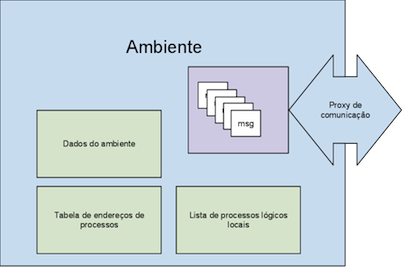
\includegraphics{Environment_1.png}}
  \caption{A arquitetura interna de um \textit{environment}.}
\label{fig:environment_1}
\end{figure}

A estrutura interna de dados do ambiente é a representação de todos as variáveis pertencentes ao \textit{environment}. Dados como o endereço físico (IP:PORT) do ambiente na rede, endereço lógico do ambiente e quantidade de processos residentes no \textit{environment} são armazenadas neste espaço.

Um \textit{environment} possui um endereço lógico único em toda o ciclo de vida da simulação, denominado \textit{Unique Environment Identifier} - \textit{UEI}. Este endereço é um número natural, e o representa no sistema de simulação.

A comunicação entre dois \textit{environmets} se dá através seu endereço físico na rede (IP:PORT). Tal inflexibilidade é justificada quando assumimos que um \textit{environment} tem todo o seu ciclo de vida atrelado a um mesmo nó físico do sistema.

\subsection{\textit{Proxy}}

O \textit{proxy} é a camada do \textit{environment} que é responsável por toda troca de mensagem entre os processos. O \textit{proxy} atua de maneira distinta em troca de mensagens entre processos que convivem no mesmo ambiente e entre trocas de mensagens entre processos que se situam em ambientes distintos. As distinções entre trocas de mensagens internas e externas serão tratadas na seção~\ref{troca_mensagens}

O \textit{proxy} também é o único canal por onde os processos recebem mensagens providas de fora do ambiente. Toda mensagem recebida pelo proxy é identificada pelo enreço lógico do processo destinatário. Cabe ao proxy converter este enedeço lógico em seu endereço físico e encaminhar a mensagem ao destino.

Como todo o tratamento de envio e recebimento de mensagens deve ser não-blocante, o \textit{proxy} deve operar de maneeira assíncrona aos demais módulos do \textit{environment}.

\subsection{Tabela de endereços de processos}

A tabela de endereços dos processos é uma lista associativa que possui informações básicas de endereços e status dos processos existentes. Esta tabela contém informações não apenas dos processos residentes no \textit{environment} em questão, mas também dados de dos processos residentes em outros ambientes de simulação pertencentes ao mesmo sistema. Esses dados são necessários para se prover a comunicação entre processos residentes em ambientes distintos.

Todo processo possui um endereço lógico e um endereço físico. O seu endereço lógico é único em toda a simulação, e não muda mesmo se o processo migrar de um ambiente para outro. Já o seu endereço físico depende do \textit{environment} em que ele está em um determinado momento. A tradução de endereço lógico para endereço físico se faz utilizando a tabela de endereço de processos. Após cada migração, o \textit{proxy} referente ao ambiente que recebeu o processo que migrou responsável por enviar mensagem aos demais ambientes, atualizando seu endereço do processo em questão.

Além de armazenar dados refrente aos endereços lógicos e físicos dos processos, a tabela de endereços armazena também uma variável de \textit{status} de cada processo. Os estados de um processo podem ser:

\begin{itemize}
\item Ativo: Indica que o processo se encontra neste \textit{environment} e está ativo. 
\item Ausente: Indica que o processo em questão se encontra em outro ambiente.
\item Trânsito: Indica que o processo em questão estava em um momento anterior neste ambiente e migrou para um ambiente diferente, porém ainda não atualizou a tabela de endereços com seu endereço físico atual.
\item Inativo: Indica que o processo se encontra neste ambiente, mas não está ativo.
\end{itemize}

Os estados ativo e inativo são os estados mais comuns de um processo em um sistema típico. Eles indicam que o processo em questão está, ou não, em execução naquele ambiente. Um processo em estado inativo significa que este está residente no \textit{environment} em questão, mas não está executando no momento por algum motivo não identificado. Toda mensagem recebida para ser entregue a um processo inativo será armazenada no buffer de mensagens do \textit{proxy} e deverá ser retirada posteriormente pelo processo.

O estado de trânsito indica que o processo esteve naquele \textit{environment} em algum instante do passado e que sofreu uma migração, mas seu novo endereço não foi ainda atualizado. Mais informações de como funciona a atualização de endereços durante a migração pode ser encontrado na Seção~\ref{atualizacao}.

\section{O componente \textit{process} \label{process}}

Um processo é uma unidade discreta de processamento em um sistema de simulação de eventos discretos. É ele o responsável por retirar cada evento a ser executado da fila de eventos futuros e executá-lo. A representação de um processo lógico na arquitetura aqui descrita se dá pelo objeto \textit{process}.

Um processo lógico possui duas identificações distintas no sistema: seu endereço físico em memória e seu endereço lógico no sistema de simulação. Na arquitetura deste \textit{middleware}, o processo é referenciado em uma troca de mensagens sempre pelo seu endereço lógico. Cabe ao \textit{proxy} do ambiente fazer, quando for necessário, a conversão do endereço lógico para seu equivalente endereço físico a fim de entregar a mensagem ao processo de destino.

Neste ponto a comunicação se divide em dois tipos diferentes: comunicação entre processos cohabitantes (que habitam o mesmo \textit{environment}) e comunicação de processos não-cohabitantes (\textit{environment} diferentes). Essa diferença força a utilização de meios distintos de comunicação para cada caso, porém isto é resolvido internamente pelo \textit{middleware}, deixando a comunicaçào transparente para o \textit{framework}.

Mais detalhes sobre a comunicação entre processos e a distinção entre comunicação entre processos cohabitantes e não-cohabitantes são detalhados na seção~\ref{troca_mensagens}.

\subsection{Ciclo de vida de um processo}

Um processo lógico tal como descrito pelo \textit{middleware} possui um ciclo de vida com fases bem definidas. Isso significa que a classe base a qual o usuário do \textit{middleware} extende para criar seu processo lógico já prevê, na forma de métodos abstratos, espaços onde serão implementados trechos importantes para fases específicas da vida do processo. Essas fases estão ilustradas no diagrama da Figura~\ref{fig:estados_processos}. A representação dos \textit{slots} onde serão inseridos os códigos, na forma de métodos abstrados é ilustrada na representação UML da Figura~\ref{fig:process_uml}.

O primeiro método invocado automaticamente pelo processo na sua criação é o método on\_create. Este método é chamado apenas uma única vez em todo o ciclo de vida do processo lógico e trata das rotinas de inicialização do processo. Este método pode ser visto de maneira análoga ao construtor de uma classe, na programação orientada à objetos. Imediatamente após executar o código contido no método on\_create, o próximo méto invocado automaticamente pelo sistema é o método run.

O método run é onde o corpo da simulação deve estar implementado. É neste ponto do código onde, em um laço repetitivo, São retirados os eventos da fila de eventos futuros para a sua execução. Vale ressaltar que como descreve \cite{RIBEIROALVES}, o processo de se retirar eventos da fila de eventos futuros para execução não pode ser feito na forma de um laço de repetição convencional, pois tornaria a execução do método não-preemptiva (bloqueando a execução neste laço). 

A solução apontada por \cite{RIBEIROALVES} é a de, após realizar a execução de um evento da fila de eventos futuros, enviar uma mensagem para si mesmo agendando a execução do próximo evento. Isso permitiria a intercalação entre mensagens para executar um novo evento com mensagens externas, trazendo novos eventos, mensagens de sincronização, etc.

Cabe aqui ressaltar que a ação de retirar um evento da fila de eventos futuros é implementada internarmente na estrutura do \textit{framework}, e o seu usuário não precisa explicitamente descrever tal tarefa.

\begin{figure}
  \centerline{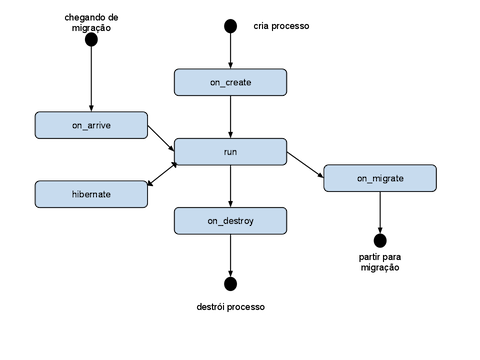
\includegraphics{estados_processos.png}}
  \caption{Ciclo de vida de um processo lógico.}
\label{fig:estados_processos}
\end{figure}

\begin{figure}
  \centerline{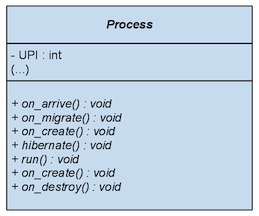
\includegraphics{process_uml.png}}
  \caption{Representação em diagrama de classe do componente \textit{process}.}
\label{fig:process_uml}
\end{figure}

Os demais métodos invocados automaticamente pelo sistema são on\_migrate, invocado antes da migração. on\_arrive, invocado assim que o processo chega no destino. hibernate, invocado quando um processo é adormecido e on\_destroy, invocado ao se destruir um processo lógico.

Naturalmente a classe \textit{Process} comporta a criação de demais métodos além destes pré-estipulados, porém apenas estes métodos são executados de maneira automática pelo \textit{middleware} em ocasiões especiais.

\subsection{Serialização de um processo}

Serialização é a capacidade que um objeto possui de converter sua estrutura interna de dados em uma representação binária ou codificada em texto, a fim de se armazenar ou reutilizar posteriormente

Um processo deve possuir a propriedade de ser serializado quando conveniente. A serialização de um processo se dá internamente no \textit{framework} a partir de chamadas do \textit{middleware}. Ao usuário cabe garantir que todo o código escrito seja serializável.

\section{Migração de processos \label{migracao}}

Uma das principais características propostas pelo \textit{middleware} de comunicação que compões este trabalho á a possibilidade de que processos lógicos migrem de seu nó de origem para um diferente nó do sistema a fim de, por exemplo, prover um balanceamento de cargas através do sistema. Para que isso ocorra, naturalmente, o nó destino deve possuir uma instância ativa de um \textit{environment} capaz de gerenciar a continuidade da vida do processo em questão.

Para que a migração ocorra, uma série de ações ocorre em uma determinada ordem, para garantir a integridade do sistema durante este processo. A sequência de eventos para uma migração de um processo pode ser descrita como a seguir:

\begin{enumerate}
\item O estado do processo (a ser migrado) na tabela de endereços é modificade de Ativo para Trânsito.
\item O método on\_migrate é invocado ainda no ambiente de origem do processo.
\item O processo a ser migrado é serializado pelo \textit{environment} de origem e enviado para o ambiente de destino.
\item O ambiente de destino recebe o processo serializado e o desserializa, tornando-o um novo objeto em memória, mas mantendo os dados originais do processo.
\item O ambiente de destino atualiza o estado do processo em sua tabela local de Ausente para Inativo.
\item O ambiente de destino envia uma mensagem para o ambiente de origem indicando que o processo chegou, e qual o novo endereço físico do processo.
\item O \textit{environment} de origem atualiza o estado do processo para Ausente. Atualiza também o endereço físico do processo na tabela de endereços.
\item O processo executa o método on\_arrive no ambiente de destino.
\item O \textit{environment} muda o status do processo de Inativo para Ativo.
\item Por fim, o processo recupera todas as mensagens do buffer de mensagens do proxy de comunicação, resgatando eventuais mensagens recebidas enquanto o seu estado era Inativo.
\item O processo, já em estado ativo, executa o método run.
\item Uma mensagem em \textit{broadcast} é enviado a todos os \textit{environment}, sinalizando o novo endereço físico correspondente à aquele processo acaba de migrar. As tabelas de endereços são então atualizadas.
\end{enumerate}

Assim que o processo termina o ciclo de ações de migração ele está apto a continuar a simulação do ponto onde parou no ambiente antigo. Isto se dá poque o processo foi serializado e todos os dados foram mantidos tais como estavam instantes antes da migração.

\subsection{Atualização da tabela de endereços dos processos \label{atualizacao}}

Uma vez que um processe migra de um \textit{environment} para outro, instantes após a migração apenas os dois ambientes envolvidos na transação possuem os dados atualizados referentes ao processo que migrou. Todo ambiente difente dos envolvidos no processo de migração possuem em suas tabelas de endereços de processos dados desatualizados quanto à sua localização, portanto, enviariam mensagens para o ambiente antigo, ao qual o processo em questão não mais pertence.

Ao receber uma mensagem destinada a um processo que não mais o habita, um \textit{environment} (que possui o endereço atualizado do processo em questão), redireciona a mensagem ao proxy do ambiente que possui atualmente este processo. Porém, isso inclui mais um intermediário no processo de transmissão de mensagens. Sendo assim, duas ações, em momentos distintos, são efetuadas para garantir a atualização das tabelas de endereços de processos. Primeiro, o antigo \textit{host} do processo, ao receber a mensagem, além de repassa-la ao atual \textit{host} também devolve uma mensagem para o remetente da mensagem, notificando-o que o endereço do ambiente que contém o processo mudou, e atualiza este endereço.

Em um momento distinto, uma segunda ação de sincronismo de tabelas é disparada. Esta ação é iniciada de forma idependente por cada \textit{environment}, enviando uma mensagem para os demais ambientes, notificando-os de quais processos lógicos encontram-se em seu poder. Isto garante uma atualização constante das diversas tabelas de endereços de processos existente na simulação.

\section{Troca de mensagens \label{troca_mensagens}}

No modelo de comunicação implementado pelo \textit{middleware} de comunicação, a troca de mensagem entre dois processos lógicos ocorre de maneira distinta, dependendo se os processos cohabitam um mesmo ambiente ou não.

Caso os processos residam no mesmo ambiente, é utilizada a chamada comunicação direta, onde a mensagem é diretamente transmitida de um processo para o seu destino. Porém, quando um processo deseja enviar uma mensagem à um processo que habita um \textit{environment} distinto, a mensagem é primeiramente encaminhada ao \textit{proxy} do \textit{environment} do processo remetente da mensagem, e cabe a este redirecionar a mensagem ao seu destino. A este processo dá-se o nome de comunicação indireta.

\subsection{Comunicação local direta}

A comunicação direta ocorrem quando tanto o processo lógico que envia mensagem quanto o destinatário habitam um mesmo ambiente no sistema de simulação. Esta comunicação se dá através do endereço físico do processo destinatário, sem a necessidade de intervenção do \textit{proxy} do ambiente para redirecionar a mensagem.

\begin{figure}
  \centerline{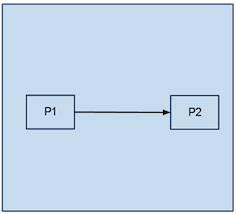
\includegraphics{communication_superdirect.png}}
  \caption{Comunicação direta \textit{process-process}.}
\label{fig:direta_mesmo}
\end{figure}

Quando o processo P1 deseja enviar uma mensagem ao processo P2, o processo remetente possui o endereço lógico do processo destinatário. Este processo invoca um método interno de envio de mensagem que, por sua vez, invoca o \textit{proxy} do sistema a fim de traduzir o endereço lógico em um endereço físico.

De maneira prática, ao se invocar o método de envio de mensagem do processo P1 este recebe internamente do \textit{proxy} do sistema uma função invocável que é responsável por enviar a mensagem ao destinatário. No caso da comunicação direta, a função devolvida pelo proxy possui o endereço físico em memória do processo destinatário, e é capaz de enviar a mensagem diretamente para ele, sem uma nova intervençao do \textit{proxy}.

Todas estas ações são realizadas internamente pelo \textit{middleware} de comunicação, e não necessitam de intervenção externa em momento algum.

\subsection{Comunicação indireta}

Quando a comunicação é feita por dois processos lógicos residentes em diferentes \textit{environments} (e por consequência, em máquinas distintas da rede) a comunicação se dá através dos \textit{proxies} dos \textit{environments}. O fluxo de comunicação é ilustrada de maneira simplificada na Figura~\ref{fig:indireta}.

Quando o processo P1 deseja enviar uma mensagem ao processo P3, e estes habitam ambientes distintos no sistema, ao se executar o método para enviar uma mensagem, o \textit{proxy} responsável pelo processo P1 identifica que o processo P3 não pertence ao mesmo ambiente. Assim, internamente o proxy devolve uma função ao processo P1 (de maneira idêntica ao que ocorre na comunicação direta), porém com a diferença que esta função não possui o endereço físico do processo P3, mas sim o endereço físico do \textit{proxy} responsável por P3 (este endereço é obtido através da tabela de endereços e do endereço lógico de P3).

Uma vez que o processo P1 recebeu (de maneira automática e interna ao \textit{middleware}) o endereço físico do \textit{proxy} responsável pelo processo P3, a mensagem é então enviada ao ambiente de destino e, uma vez entregue, é redirecionada pelo seu \textit{proxy} para o processo P3.

\begin{figure}
  \centerline{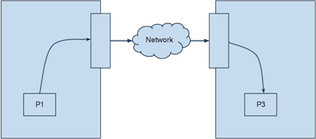
\includegraphics{Communication_indireta.png}}
  \caption{Comunicação indireta \textit{proxy-process}.}
\label{fig:indireta}
\end{figure}

A adoção da interferência dos \textit{proxies} na transmissão das mensagens entre os processos pode parecer a princípio um ítem custoso e dispensável no sistema, uma vez que cada processo poderia abrigar sua própria tabela de endereços e fazer a tradução de endereços físicos para lógicos de maneira direta. Porém isso elevaria a quantidade de tabelas a se atualizar em caso de migraçào de processos.

Em um modelo onde cada processo resolveria independentemente a tradução de endereço lógigo para o seu correspondente físico para o envio de mensagens, a quantidade de tabelas de endereços seria proporcional à quantidade de processos lógicos existentes no sistema (e não proporcional à quantidade de ambientes, como é na arquitetura proposta). Isso elevaria consideravelmente a quantidade de tabelas de endereço a se atualizar no caso de uma possível migração.

\section{Comunicação grupal}

Por definição agentes móveis não suportam comunicação grupal. Uma das lacunas de se utilizar agentes móveis para a implementação de um framework de simulação distribuída é justamente a ausência de um mecanismo nativo de comunicação grupal, necessário para a implementação do protocolo \textit{Rollback} Solidário.

Uma alternativa para este problema seria o envio de múltiplas mensagens para cada \textit{environment} presente no sistema, o que seria uma solução parcial, pois a medida que aumenta-se a quantidade de nós existentes no sistema, aumenta-se a quantidade de mensagens a serem enviadas.

A arquitetura do \textit{middleware} proposto resolve este problema em dois níveis: primeiramente existe o envio de mensagens em broadcasta que atingem simultaneamente todos os \textit{environments} do sistema. Em seguida cada environment envia uma mensage física local para cada processo. Como a comunicação entre \textit{environment} e processo é local, não há sobrecarga na rede.
